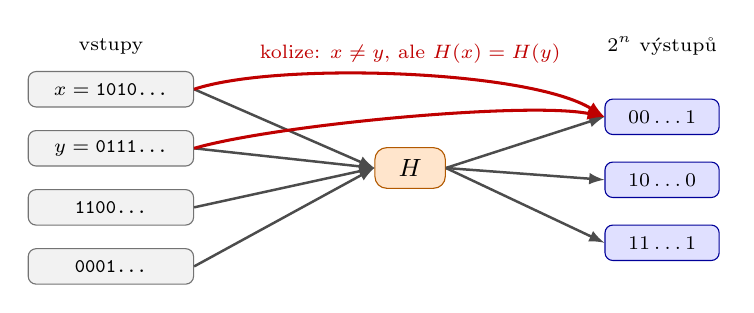
\begin{tikzpicture}[
    x=1cm,y=1cm,
    >=latex,
    arrow/.style={->, >=latex, line width=0.9pt, draw=black!70},
    msg/.style={
        rounded corners=1mm,
        draw=black!55,
        fill=black!5,
        minimum width=2.1cm,
        minimum height=0.45cm,
        font=\scriptsize
    },
    hash/.style={
        rounded corners=1mm,
        draw=blue!60!black,
        fill=blue!12,
        minimum width=1.45cm,
        minimum height=0.45cm,
        font=\scriptsize
    }
]
    
    \node[msg] (x1) at (-3.8,1.0) {\(x=\texttt{1010\ldots}\)};
    \node[msg] (x2) at (-3.8,0.25) {\(y=\texttt{0111\ldots}\)};
    \node[msg] (x3) at (-3.8,-0.5) {\(\texttt{1100\ldots}\)};
    \node[msg] (x4) at (-3.8,-1.25) {\(\texttt{0001\ldots}\)};
    
    \node[font=\scriptsize] at (-3.8,1.55) {vstupy};
    
    \node[hash] (h1) at (3.2,0.65) {\(00\ldots 1\)};
    \node[hash] (h2) at (3.2,-0.15) {\(10\ldots 0\)};
    \node[hash] (h3) at (3.2,-0.95) {\(11\ldots 1\)};
    
    \node[font=\scriptsize] at (3.2,1.55) {\(2^n\) výstupů};
    
    \node[
        rounded corners=1.5mm,
        draw=orange!70!black,
        fill=orange!20,
        font=\small,
        inner xsep=3mm,
        inner ysep=1.5mm
    ] (H) at (0,0) {\(H\)};
    
    \draw[arrow] (x1.east) -- (H.west);
    \draw[arrow] (x2.east) -- (H.west);
    \draw[arrow] (x3.east) -- (H.west);
    \draw[arrow] (x4.east) -- (H.west);
    
    \draw[arrow] (H.east) -- (h1.west);
    \draw[arrow] (H.east) -- (h2.west);
    \draw[arrow] (H.east) -- (h3.west);
    
    % zvýrazněná kolize
    \draw[->, >=latex, line width=1.1pt, draw=red!75!black]
        (x1.east) .. controls (-1.7,1.35) and (1.5,1.25) .. (h1.west);
    \draw[->, >=latex, line width=1.1pt, draw=red!75!black]
        (x2.east) .. controls (-1.7,0.55) and (1.5,0.85) .. (h1.west);
    
    \node[font=\scriptsize, text=red!75!black] at (0,1.45)
        {kolize: \(x\neq y\), ale \(H(x)=H(y)\)};
    
\end{tikzpicture}
